\section{Experiments}
Our generalised shapelet transform, contrasted with the classical shapelet transform, has two extra degrees of freedom: the choice of interpolation scheme $\iota$, and the choice of discrepancy function $\pi^A_S$. In our experiments, we consider $\pi^A_S$ given by either of equations \eqref{eq:learnt-discrepancy} or \eqref{eq:logsignature-discrepancy}. Meanwhile, we take $\iota$ to be piecewise linear interpolation, because efficient algorithms for computing the logsignature transform only exist for piecewise linear paths \cite{signatory}.

TODO: we need to consider more disrepancy functions than this.


\subsection{The UEA (Multivariate) Time-Series Archive}
We begin by comparing the classification performance of the old method of shapelets to our new `generalised' approach for which we consider three learnt metrics: a standard L2-metric, an learnt metric and a logsig-3-diagonal. We evaluate the methods on a subset of the UEA time-series archive \cite{bagnall2018uea}. This contains a wide range of multivariate time-series classification problems from various fields with significant differences in time-series length, number of classes, and amount of training data. The full collection contains 30 datasets, however due to algorithm run-time constraints we have considered a subset of these ensuring they still contain significant variation. The statistics of these dataset are given in Table \ref{} of the Appendix.

The results are given in Table \ref{tab:uea_comparison_results}. We see improved performance from the old shapelet method in ? of ? cases. Whats more, we see there are datasets for which the optimal accuracy is achieved with a learnt metric and the logsignature discrepancy. These results, whilst not extensive, show the feasibility of improving performance by choosing a discrepancy tailored to the structure of the data as opposed to a simple euclidean distance metric.
\begin{table}[ht]
    \centering
    \caption{}
    \label{tab:uea_comparison_results}
    \begin{tabular}{lccc}
\toprule
{} &  logsig-3diagonal &  L2-diagonal &   old \\
\midrule
AtrialFibrillation &             0.333 &        0.333 & 0.467 \\
BasicMotions       &             1.000 &        0.950 & 0.975 \\
ERing              &             0.574 &        0.919 & 0.737 \\
FingerMovements    &             0.450 &        0.560 & 0.490 \\
JapaneseVowels     &             0.646 &        0.914 & 0.949 \\
Libras             &             0.739 &        0.661 & 0.661 \\
NATOPS             &                 - &        0.861 &     - \\
PenDigits          &             0.967 &        0.956 & 0.956 \\
RacketSports       &             0.717 &        0.717 & 0.605 \\ 
\midrule
Wins &                 3 &            4 &    2 \\
\bottomrule
\end{tabular}

\end{table}


\subsubsection{Algorithm Interpretability}
TODO: It would be good to include more than 4 images here, we could include one of each number corresponding to the largest logreg value for that class and plot a row from 0-9 for each class. This would actually save space and hopefully demonstrate the interpretable aspect much better. It will also look like we havent just picked out two nice ones and two bad ones if we note they were the largest coefficient for each class.

Here we explore the effect of the inclusion of the regularisation term from Equation \cite{eq:interpretable_reg} on shapelet interpretability. Recall that the term was chosen to ensure the resulting shapelets are `close', in the sense of the chosen discrepancy, to some subsample of the training data giving a natural interpretability as representing those such subsamples of the data. To examine this we consider the PenDigits dataset where participants were asked to write down a number from 0-9 and the goal is to classify the intended digit. In Figure \ref{fig:pendigits} we plot two of the learnt shapelets for both the old algorithm (top) and the regularised algorithm (bottom). For the regularised algorithm one could immediately guess that the first shapelet is designed to distinguish the number two, as it looks like the top half of the number two, and the second clearly looks like a number 7. By looking at the coefficients of the logistic regression, one does indeed find that these are the main classes that these shapelets aim to discriminate. On the other hand it is much less clear what is represented by the old shapelets, it turns out these also aim to represent a two and a seven but it is less clear that this is the case.

We chose PenDigits here because it is easy to understand visually what the shapelet represents. In general this is not the case, but provided we can make sense of isolated subintervals of the time-series, then the generated results will be interpretable in this context.
\begin{figure}[ht]
    \begin{subfigure}[b]{0.5\linewidth}
        \centering
        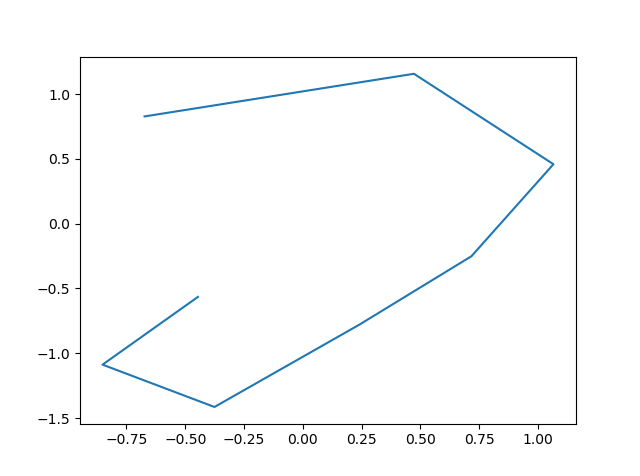
\includegraphics[width=0.75\linewidth]{images/pendigits/old_2}
        \caption{Old 2}
        \label{fig:a}
    \end{subfigure}
    \begin{subfigure}[b]{0.5\linewidth}
        \centering
        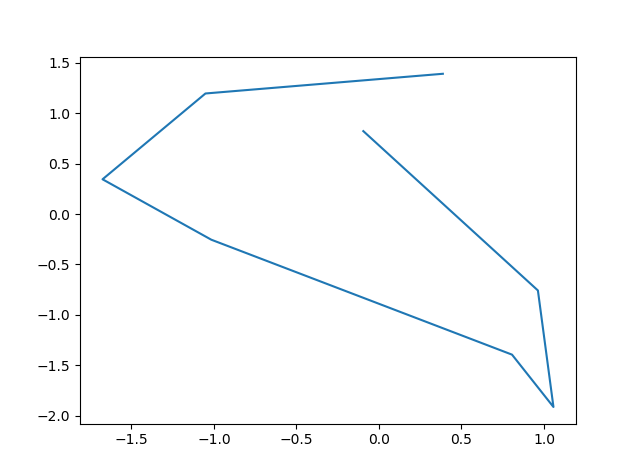
\includegraphics[width=0.75\linewidth]{images/pendigits/old_7}
        \caption{Old 7}
        \label{fig:b}
    \end{subfigure}
    \begin{subfigure}[b]{0.5\linewidth}
        \centering
        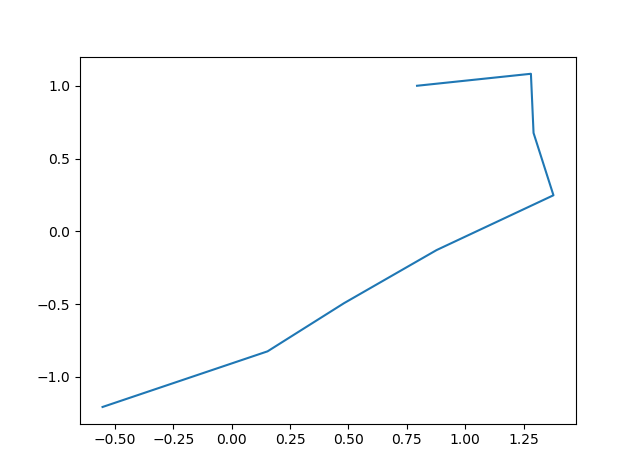
\includegraphics[width=0.75\linewidth]{images/pendigits/new_2}
        \caption{New 2}
        \label{fig7:c}
    \end{subfigure}
    \begin{subfigure}[b]{0.5\linewidth}
        \centering
        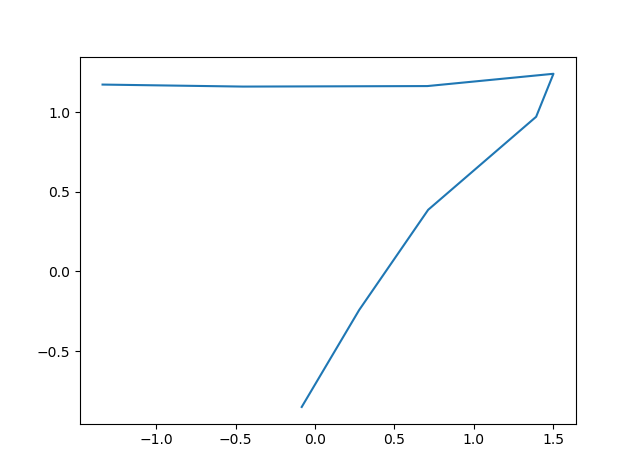
\includegraphics[width=0.75\linewidth]{images/pendigits/new_7}
        \caption{New 7}
    \end{subfigure}
    \caption{Learnt shapelets from the PenDigits dataset with the old algorithm (top) and the new algorithm (bottom).}
    \label{fig:pendigits}
\end{figure}


\subsubsection{Missing Data and Length Ablation}
We now demonstrate both the ability of the proposed framework to handle partially observed data, as well as show the effectiveness of having learnable shapelet lengths.
\begin{table}[ht]
    \caption{}
    \label{tab:uea_noise}
    \centering
    \begin{tabular}{lccc}
\toprule
& \multicolumn{3}{c}{\textbf{Discrepancy}} \\
\textbf{Dataset} &  L2-diagonal-False &   L2-diagonal-True &                old \\
\midrule
BasicMotions3     &  0.360 $\pm$ 0.175 &  0.320 $\pm$ 0.157 &  0.520 $\pm$ 0.262 \\
BasicMotions30    &  0.250 $\pm$ 0.000 &  0.280 $\pm$ 0.067 &  0.360 $\pm$ 0.213 \\
BasicMotions9     &  0.365 $\pm$ 0.139 &  0.325 $\pm$ 0.075 &  0.450 $\pm$ 0.202 \\
FingerMovements3  &  0.496 $\pm$ 0.009 &  0.536 $\pm$ 0.051 &  0.498 $\pm$ 0.054 \\
FingerMovements30 &  0.512 $\pm$ 0.029 &  0.506 $\pm$ 0.065 &  0.522 $\pm$ 0.044 \\
FingerMovements9  &  0.504 $\pm$ 0.047 &  0.510 $\pm$ 0.031 &  0.480 $\pm$ 0.041 \\
JapaneseVowels3   &  0.812 $\pm$ 0.158 &  0.725 $\pm$ 0.195 &  0.857 $\pm$ 0.027 \\
JapaneseVowels30  &  0.419 $\pm$ 0.221 &  0.209 $\pm$ 0.081 &  0.611 $\pm$ 0.175 \\
JapaneseVowels9   &  0.432 $\pm$ 0.221 &  0.556 $\pm$ 0.324 &  0.805 $\pm$ 0.041 \\ 
\midrule
Wins &                  0 &                 2 &    7 \\
\bottomrule
\end{tabular}

\end{table}


\subsection{Speech Commands}
Finally we examine the performance on the speech commands dataset \ref{warden2018speech} which includes a selection of one-second audio files with each representing a single spoken word. The aim is to build a model to detect the word that has been spoken. We chose this dataset as it is significantly larger than any in the UEA archive so as to demonstrate that the method is not restricted to these (relatively) small datasets. We do reiterate that the computational cost of shapelet methods is high in comparison to other more traditional deep-learning approaches and so can make datasets such as this prohibitive, in particular, it is why we have left the logsig-3 discrepancy out of our analysis in this instance as it takes significantly longer to train compared with the L2 methods.
\begin{table}[ht]
    \caption{Classification accuracy for old shapelets and new shapelets on the Speech Commands dataset.}
    \label{tab:speech_commands}
    \centering
    \begin{tabular}{cc}
\toprule
\multicolumn{2}{c}{Discrepancy} \\
Old &  L2 \\
\midrule
- & - \\
- & - \\
\bottomrule
\end{tabular}

\end{table}

\subsubsection{Interpretability of Speech Commands}
Pray for me.

